%\documentclass{article}
\documentclass[10pt,a4paper]{article}
\usepackage[top=30pt,bottom=30pt,left=48pt,right=46pt]{geometry}

\usepackage[utf8]{inputenc}

\title{Book of Solutions}
\author{C Thierfelder}
\date{May 2020}

\usepackage{natbib}

%MATH
\usepackage{amsmath}
\usepackage{amsfonts}

%PAGELAYOUT
\usepackage{a4wide}

%GRAPHICS
\usepackage{graphicx}
\usepackage[dvipsnames]{xcolor}
\usepackage{tikz}
\usetikzlibrary{shapes}
\usetikzlibrary{plotmarks}

%HYPERLINKS
\usepackage{hyperref}
\hypersetup{
    colorlinks=true,
    linkcolor=blue,
    filecolor=magenta,      
    urlcolor=cyan,
}

\usepackage[shortlabels]{enumitem}

\begin{document}

\maketitle

\section{Introduction}
There is a theory which states that if ever anyone discovers exactly what the Universe is for and why it is here, it will instantly disappear and be replaced by something even more bizarre and inexplicable.
There is another theory which states that this has already happened.

\begin{figure}[h!]
\centering
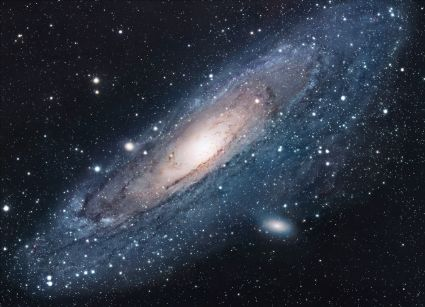
\includegraphics[scale=1.7]{universe}
\caption{The Universe}
\label{fig:universe}
\end{figure}

\newpage
\tableofcontents

%SECTION_NUMBERING
\setcounter{secnumdepth}{2}

\newpage

\section{Primer special relativity}
Definition of line element
\begin{align}
    ds^2 &= dx^\mu dx_\nu = \eta_{\mu\nu}dx^\mu dx^\nu\\
        &= dx^T\eta dx
\end{align}
Definition of Lorentz transformation
\begin{align}
    dx^\mu = \Lambda^\mu_{\;\nu}dx^\nu
\end{align}
By postulate the line element $ds$ is invariant under Lorentz transformation
\begin{align}
    ds^2 &= \eta_{\mu\nu}dx^\mu dx^\nu\\
    &\stackrel{!}{=} \eta_{\alpha\beta}\Lambda^\alpha_{\;\mu}dx^\mu \Lambda^\beta_{\;\nu}dx^\nu\quad\rightarrow\quad \eta_{\mu\nu} = \eta_{\alpha\beta}\Lambda^\alpha_{\;\mu} \Lambda^\beta_{\;\nu}
\end{align}
or analog
\begin{align}
    ds^2 &= dx^T\eta dx\\
    &\stackrel{!}{=} (\Lambda dx)^T\eta (\Lambda dx)\\
    &= dx^T\Lambda^T\eta \Lambda dx\quad\rightarrow\quad \eta = \Lambda^T\eta\Lambda
\end{align}
Observation with the eigentime $d\tau=ds/c$ and 3-velocity $dx^i = v^i dt$
\begin{align}
    \frac{ds^2}{d\tau^2}=c^2&=c^2\frac{dt^2}{d\tau^2}-\frac{dx^i}{dt}\frac{dx_i}{dt}\left(\frac{dt}{d\tau}\right)^2\\
    1&=\frac{dt^2}{d\tau^2}\left(1-\frac{v^iv_i}{c^2}\right)\quad\rightarrow\quad\frac{dt}{d\tau}\equiv\gamma=\left(\sqrt{1-\frac{v^2}{c^2}}\right)^{-1}
\end{align}
Definition of 4-velocity with 3-velocity $d\vec{x} = \vec{v} dt$
\begin{align}
    u^\mu\equiv\frac{dx^\mu}{d\tau}&=\frac{dx^\mu}{dt}\frac{dt}{d\tau}=\quad\rightarrow\quad u^\mu u_\mu=\eta_{\mu\nu}\frac{dx^\mu}{\tau} \frac{dx^\nu}{\tau}=\frac{1}{\tau^2}ds^2=c^2\\
    &=(c,\vec{v})\gamma
\end{align}
Object moving in $x$ direction with $v$ meaning $dx=v\cdot dt$ compared to
rest frame $dx'=0$
\begin{align}
    c^2dt'^2=ds^2 &= c^2dt^2- v^2 dt^2\\
    &=c^2dt^2\left(1-\frac{v^2}{c^2}\right)\\
    dt'=\frac{ds}{c}\equiv d\tau&=dt\sqrt{1-\frac{v^2}{c^2}}=\frac{dt}{\gamma}
\end{align}
Definition 4-momentum
\begin{align}
    p^\mu \equiv mu^\mu=(\gamma mc,\gamma m\vec{v})\quad&\rightarrow\quad p^\mu p _\mu=m^2u^\mu u_\mu=m^2c^2\\
    &\rightarrow\quad (p^0)^2-p^ip_i=m^2c^2\\
    &\rightarrow\quad p^0=\sqrt{m^2c^2+\vec{p}^2}
\end{align}

\section{Quantum Field Theory}
\subsection{{\sc Srednicki} - Quantum Field Theory}
\subsubsection{Problem 6.1 - Path integral in quantum mechanics}

\section{Quantum Gravity}
\subsection{{\sc Ammon, Erdmenger} - Gauge/Gravity Duality - Foundations and Applications}
The authors use $d-1$ spacial dimension and the sign convention 
\begin{align}
\eta_{\mu\nu}=diag(-1,1,...,1)
\end{align}
which implies 
\begin{align}
    \square&=\partial^\mu\partial_\mu=-\partial_t^2+\triangle\\
    kx&=-k^0x^0+\vec{k}\vec{x}
\end{align}
and results in a minus sign in the KG equation.

\subsubsection{Problem 1.1.1 - Fourier representation of free scalar field}
Ansatz (because KG equation looks quite similar to wave equation) $\phi(x)=a\cdot e^{ikx}$ with $x^\mu=(t,\vec{x})$, $k^\mu=(\omega,\vec{k})$ and $a\in\mathbb{C}$ meaning 
\begin{align}
    e^{ikx}\equiv e^{ik^{\mu}x_{\mu}}=e^{i\eta_{\mu\nu}k^{\mu}x^{\nu}}=e^{i(-k^0x^0+\vec{k}\vec{x})}
\end{align}
Inserting into the equation of motion
\begin{align}
    (\square - m^2)\phi(x)&=(\partial^t\partial_t + \triangle - m^2)\phi(x)\\
    &=a(-\partial_t^2 + \triangle - m^2)e^{i(-\omega t+\vec{k}\vec{x})}\\
    &=a\left(\omega^2 + i^2\vec{k}^2 - m^2\right)e^{i(-\omega t+\vec{k}\vec{x})}=0 
\end{align}
This implies $\omega^2-\vec{k}^2-m^2=0$ and therefore $\omega_k\equiv\omega=\sqrt{\vec{k}^2+m^2}$. One particular solution is therefore $\phi(x)=a\cdot e^{ikx}|_{k^0=\omega_k}$. The general solution is then given by a superposition
\begin{align}
    \phi(x)=\int d^{d-1}\vec{k}\left[a(\vec{k})e^{ikx}\right]
\end{align}
to ensure a real valued $\phi{x}$ we add the conjugate complex solution
\begin{align}
    \phi(x)=\int d^{d-1}\vec{k}\left[a(\vec{k})e^{ikx} + a^*(\vec{k})e^{-ikx}\right].
\end{align}
The factor $(2\pi)^{1-d}/2\omega_k$ can be absorbed into $a(k)$.

\subsubsection{Problem 1.1.2 - Lagrangian of self-interacting scalar field}
The Lagrangian is then
\begin{align}
    \mathcal{L}&=\mathcal{L}_\text{free}+\mathcal{L}_\text{int}\\
                &=-\frac{1}{2}\eta^{\mu\nu}\partial_\mu\phi(x)\partial_\nu\phi(x)-\frac{1}{2}m^2\phi(x)^2-\frac{g}{4!}\phi(x)^4.
\end{align}
with the Euler-Lagrange equations
\begin{align}
    \partial_\alpha\left(\frac{\partial\mathcal{L}}{\partial(\partial_\alpha\phi)}\right)-\frac{\partial\mathcal{L}}{\partial\phi}=0.
\end{align}
Therefore
\begin{align}
    \partial_\alpha\left(\frac{\partial\mathcal{L}}{\partial(\partial_\alpha\phi)}\right)
    &=\partial_\alpha\left(-\frac{1}{2}\eta^{\mu\nu}[\delta_{\mu\alpha}\partial_\nu\phi+\partial_\mu\phi\delta_{\nu\alpha}]\right)\\
    &=\partial_\alpha\left(-\frac{1}{2}\eta^{\alpha\nu}\partial_\nu\phi-\frac{1}{2}\eta^{\mu\alpha}\partial_\mu\phi\right)\\
    &=-\partial_\alpha\left(\eta^{\alpha\beta}\partial_\beta\phi\right)\\
    &=-\partial^\beta\partial_\beta\phi\\
    &=-\square\phi
\end{align}
and
\begin{align}
    \frac{\partial\mathcal{L}}{\partial\phi} = -m^2\phi-\frac{g}{3!}\phi^3.
\end{align}

The relevant term in the Euler-Lagrange equations is $\partial\mathcal{L}_\text{int}/\partial\phi=-g\phi^3/3!$. The modified equation of motion is therefore
\begin{align}
    (\square - m^2)\phi(x)-\frac{g}{3!}\phi(x)^3=0
\end{align}

\subsubsection{Problem 1.1.3 - Complex scalar field }
\begin{align}
    \mathcal{L}_\text{free}&=-\partial_\mu\phi^*\partial^\mu\phi-m^2\phi^*\phi\\
    &=-\eta^{\mu\nu}\partial_\mu\phi^*\partial_\nu\phi-m^2\phi^*\phi\\
    &=-\frac{1}{2}\eta^{\mu\nu}\partial_\mu(\phi_1-i\phi_2)\partial_\nu(\phi_1+i\phi_2)-\frac{1}{2}m^2(\phi_1^2+\phi_2^2)\\
    &=-\frac{1}{2}\eta^{\mu\nu}\left(
    \partial_\mu\phi_1\partial_\nu\phi_1
    +i\partial_\mu\phi_1\partial_\nu\phi_2
    -i\partial_\mu\phi_2\partial_\nu\phi_1
    +\partial_\mu\phi_2\partial_\nu\phi_2
    \right)-\frac{1}{2}m^2(\phi_1^2+\phi_2^2)\\
    &=-\frac{1}{2}\eta^{\mu\nu}\left(\partial_\mu\phi_1\partial_\nu\phi_1+\partial_\mu\phi_2\partial_\nu\phi_2\right)-\frac{1}{2}m^2(\phi_1^2+\phi_2^2)\\
    &=-\frac{1}{2}\eta^{\mu\nu}\partial_\mu\phi_1\partial_\nu\phi_1-\frac{1}{2}m^2\phi_1^2
    -\frac{1}{2}\eta^{\mu\nu}\partial_\mu\phi_2\partial_\nu\phi_2-\frac{1}{2}m^2\phi_2^2\\
    &=\mathcal{L}_\text{free1}+\mathcal{L}_\text{free2}
\end{align}

Equations of motion for $\phi$ and $\phi^*$ are given by
\begin{align}
    \partial_\alpha\left(\frac{\partial\mathcal{L}}{\partial(\partial_\alpha\phi^*)}\right)-\frac{\partial\mathcal{L}}{\partial\phi^*}=0\\
    %
    -\partial_\mu\partial^\mu\phi+m^2\phi=0\\
    (\square-m^2)\phi=0
\end{align}
and
\begin{align}
    \partial_\alpha\left(\frac{\partial\mathcal{L}}{\partial(\partial_\alpha\phi^*)}\right)-\frac{\partial\mathcal{L}}{\partial\phi}=0\\
    %
    -\partial_\mu\partial^\mu\phi+m^2\phi^*=0\\
    (\square-m^2)\phi^*=0
\end{align}

\subsubsection{Problem 1.2.1 - Time-independence of Noether charge}
The conserved current is
\begin{align}
    \partial_\mu\mathcal{J}^\mu\equiv-\partial_0\mathcal{J}^0+\partial_i\mathcal{J}^i=0.
\end{align}
Spacial integration using Gauss law on the right hand side gives
\begin{align}
    \int_{\mathbb{R}^{d-1}} d^{d-1}\vec{x}\;\partial_0\mathcal{J}^0&=\int_{\mathbb{R}^{d-1}} d^{d-1}\vec{x}\;\partial_i\mathcal{J}^i\\
    %
    \partial_0\int_{\mathbb{R}^{d-1}} d^{d-1}\vec{x}\;\mathcal{J}^0&=\int_{\partial\mathbb{R}^{d-1}} dS\;\mathcal{J}^i\\
    \partial_0\mathcal{Q}&=0
\end{align}
where we used that $\mathcal{J}^i$ is vanishing at infinity.

\subsubsection{Problem 1.2.2 - Hamiltonian of scalar field}
The Lagrangian of the real free scalar field is given by 
\begin{align}
    \mathcal{L}=-\frac{1}{2}\eta^{\mu\nu}\partial_\mu\phi(x)\partial_\nu\phi(x)-\frac{1}{2}m^2\phi(x)^2.
\end{align}
The canonical momentum is therefore
\begin{align}
    \Pi &= \frac{\partial\mathcal{L}}{\partial(\partial_t\phi)}\\
    &=-\frac{1}{2}2\eta^{ti}\partial_i\phi -\frac{1}{2}2\eta^{tt}\partial_t\phi\\
    &=\partial_t\phi.
\end{align}
Using $\eta_{\mu\nu}=diag(-1,1,...,1)$ the Hamiltonian $\mathcal{H}=\Theta^{tt}=\eta^{t\nu}\Theta^t_{\;\nu}=-\Theta^t_{\;t}$ is 
\begin{align}
    \Theta^t_{\;t}
    &=-\frac{\partial\mathcal{L}}{\partial(\partial_t\phi)}\partial_t\phi+\mathcal{L}\\
    &=-\Pi\cdot\partial_t\phi+\mathcal{L}
\end{align}
and therefore
\begin{align}
    \mathcal{H}&=\Pi\partial_t\phi-\mathcal{L}\\
    &=\Pi^2-\left(-\frac{1}{2}\eta^{\mu\nu}\partial_\mu\phi(x)\partial_\nu\phi(x)-\frac{1}{2}m^2\phi(x)^2\right)\\
    &=\Pi^2-\left(\frac{1}{2}(\partial_t\phi)^2-\frac{1}{2}(\nabla\phi)^2-\frac{1}{2}m^2\phi(x)^2\right)\\
    &=\frac{1}{2}\Pi^2+\frac{1}{2}(\nabla\phi)^2+\frac{1}{2}m^2\phi(x)^2
\end{align}

\subsubsection{Problem 1.2.3 - Symmetric energy-momentum tensor}
The Lorentz transformation
\begin{align}
    \Lambda^\mu_{\;\nu}=\delta^\mu_{\;\nu}+\omega^\mu_{\;\nu}
\end{align}
implies the field transformation
\begin{align}
    \phi(x^\mu)\rightarrow\tilde\phi(x^\mu)&=\phi(x^\mu-\omega^\mu_{\;\rho}x^\rho)\\
    &=\phi(x^\mu)-\omega^\mu_{\;\rho}x^\rho\partial_\mu\phi
\end{align}
under which the Lagrangian transforms as
\begin{align}
    \mathcal{L}\rightarrow\tilde{\mathcal{L}}&=\mathcal{L}+\frac{\partial\mathcal{L}}{\partial x^\mu}dx^\mu\\
    &=\mathcal{L}-\omega^\nu_{\;\rho}x^\rho\partial_\mu(\delta^\mu_{\;\nu}\mathcal{L})\\
    &=\mathcal{L}+\partial_\mu(\omega^\nu_{\;\rho}x^\rho)\cdot(\delta^\mu_{\;\nu}\mathcal{L})-\partial_\mu(\omega^\nu_{\;\rho}x^\rho\delta^\mu_{\;\nu}\mathcal{L})\\
    &=\mathcal{L}+\omega^\nu_{\;\rho}\delta^\rho_\mu\cdot(\delta^\mu_{\;\nu}\mathcal{L})-\partial_\mu(\omega^\nu_{\;\rho}x^\rho\delta^\mu_{\;\nu}\mathcal{L})\\
    &=\mathcal{L}+\omega^\rho_{\;\rho}\mathcal{L}-\partial_\mu(\omega^\nu_{\;\rho}x^\rho\delta^\mu_{\;\nu}\mathcal{L})\\
    &=\mathcal{L}-\partial_\mu(\omega^\nu_{\;\rho}x^\rho\delta^\mu_{\;\nu}\mathcal{L})
\end{align}
where we used $\omega_{\mu\nu}=-\omega_{\nu\mu}$ meaning
\begin{align}
    \omega^\rho_{\;\rho}&=\eta^{\alpha\rho}\omega_{\alpha\rho}\\
    &=\sum_\rho\eta^{0\rho}\omega_{0\rho}+\eta^{1\rho}\omega_{1\rho}+\eta^{2\rho}\omega_{2\rho}+\eta^{3\rho}\omega_{3\rho}\\
    &=0
\end{align}    
in the last step (as $\eta$ has only diagonal elements and the diagonal elements of $\omega$ are zero). With $\delta\phi=-\omega^\mu_{\;\rho}x^\rho\partial_\mu\phi$ and $X^\mu=-\omega^\nu_{\;\rho}x^\rho\delta^\mu_{\;\nu}\mathcal{L}$ we obtain for the conserved current  
\begin{align}
    \mathcal{J}^\mu&=-\frac{\partial\mathcal{L}}{\partial(\partial_\mu\phi)}\delta\phi+X^\mu\\
    &=-\frac{\partial\mathcal{L}}{\partial(\partial_\mu\phi)}(-\omega^\nu_{\;\rho}x^\rho\partial_\nu\phi)+(-\omega^\nu_{\;\rho}x^\rho\delta^\mu_{\;\nu}\mathcal{L})\\
    &=(-\omega^\nu_{\;\rho}x^\rho)\left(-\frac{\partial\mathcal{L}}{\partial(\partial_\mu\phi)}\partial_\nu\phi+(\delta^\mu_{\;\nu}\mathcal{L})\right)\\
    &=(-\omega^\nu_{\;\rho}x^\rho)\Theta^\mu_{\;\nu}\\
    &=(-\eta^{\nu\alpha}\omega_{\alpha\rho}x^\rho)\Theta^\mu_{\;\nu}\\
    &=-\omega_{\alpha\rho}x^\rho\Theta^{\mu\alpha}\\
    &=-\frac{1}{2}\omega_{\alpha\rho}(x^\rho\Theta^{\mu\alpha}-x^\alpha\Theta^{\mu\rho})\\
    &=-\frac{1}{2}\omega_{\alpha\rho}N^{\mu\rho\alpha}
\end{align}
With $\partial_\mu\Theta^\mu_{\;\nu}=0$ and $\partial_\mu N^{\mu\nu\rho}=0$ we see
\begin{align}
    0&=\partial_\mu N^{\mu\nu\rho}\\
    &= \partial_\mu\left( x^\nu\Theta^{\mu\rho}-x^\rho\Theta^{\mu\nu}\right)\\
    &= (\partial_\mu x^\nu) \Theta^{\mu\rho}+  x^\nu (\partial_\mu \Theta^{\mu\rho}) -(\partial_\mu x^\rho)\Theta^{\mu\nu} - x^\rho (\partial_\mu\Theta^{\mu\nu})\\
    &= \delta_\mu^\nu \Theta^{\mu\rho}+  x^\nu (\partial_\mu \Theta^{\mu\rho}) -\delta_\mu^\rho\Theta^{\mu\nu} - x^\rho (\partial_\mu\Theta^{\mu\nu})\\
    &= \Theta^{\nu\rho} - \Theta^{\rho\nu}.
\end{align}
which means that the (canonical) energy-momentum tensor for Poincare invariant field theories is symmetric $\Theta^{\nu\rho} = \Theta^{\rho\nu}$.


\subsubsection{Problem 1.2.4 - Callan-Coleman-Jackiw energy-momentum tensor}
For the scalar field we have with $\mathcal{L}=-\frac{1}{2}\eta^{\alpha\beta}\partial_\alpha\phi\partial_\beta\phi-\frac{1}{2}m^2\phi^2$
\begin{align}
    \Theta^\mu_{\;\nu}&=-\frac{\partial\mathcal{L}}{\partial(\partial_\mu\phi)}\partial_\nu\phi+(\delta^\mu_{\;\nu}\mathcal{L})\\
    &=-\left(-\frac{1}{2}\eta^{\alpha\beta}\delta^\mu_{\alpha}\partial_\beta\phi-\frac{1}{2}\eta^{\alpha\beta}\partial_\alpha\phi\delta^\mu_{\beta}\right)\partial_\nu\phi +\delta^\mu_{\;\nu}\left(-\frac{1}{2}\eta^{\alpha\beta}\partial_\alpha\phi\partial_\beta\phi-\frac{1}{2}m^2\phi^2\right)\\
    &=\partial^\mu\phi\partial_\nu\phi -\frac{1}{2}\delta^\mu_{\;\nu}(\partial^\beta\phi\partial_\beta\phi+m^2\phi^2)
\end{align}
which gives in the massless case
\begin{align}
    \Theta^\mu_{\;\nu\text{, massless}}&=\partial^\mu\phi\partial_\nu\phi -\frac{1}{2}\delta^\mu_{\;\nu}\partial^\beta\phi\partial_\beta\phi\\
    \Theta_{\mu\nu\text{, massless}}&=\partial_\mu\phi\partial_\nu\phi -\frac{1}{2}\eta_{\mu\nu}\partial^\beta\phi\partial_\beta\phi
\end{align}

The new improved or Callan–Coleman–Jackiw energy-momentum tensor for a single, real, massless scalar field in $d$-dimensional Minkowski space is obtained by adding a term proportional to $(\partial_\mu\partial_\nu-\eta_{\mu\nu}\square)\phi^2$ where the proportionality constant is chosen to make the tensor traceless
\begin{align}
    T_{\mu\nu}=\partial_\mu\phi\partial_\nu\phi-\frac{1}{2}\eta_{\mu\nu}\partial_\rho\phi\partial^\rho\phi-\frac{d-2}{4(d-1)}\left(\partial_\mu\partial_\nu-\eta_{\mu\nu}\square\right)\phi^2
\end{align}
Let us now check the properties
\begin{enumerate}
    \item symmetric: obvious
    \item conserved: we use the equation of motion $\partial^\mu\partial_\mu\phi=\square\phi=0$
    \begin{align}
        \partial_\mu T^{\mu\nu}&=(\partial_\mu\partial^\mu\phi)\partial^\nu\phi+\partial^\mu\phi(\partial_\mu\partial^\nu\phi)\\
        &\quad-\frac{1}{2}\eta^{\mu\nu}\left[(\partial_\mu\partial_\rho\phi)\partial^\rho\phi + \partial_\rho\phi(\partial_\mu\partial^\rho\phi)\right]\\
        &\quad-\frac{d-2}{4(d-1)}\square\partial^\nu\phi^2+\frac{d-2}{4(d-1)}\eta^{\mu\nu}\partial_\mu\square\phi^2\\
        &=\partial^\mu\phi(\partial_\mu\partial^\nu\phi)-\frac{1}{2}\left[(\partial^\nu\partial_\rho\phi)\partial^\rho\phi + \partial_\rho\phi(\partial^\nu\partial^\rho\phi)\right]\\
        &=0
    \end{align}
    \item traceless: 
    \begin{align}
    T^\mu_{\;\mu}&=\partial^\mu\phi\partial_\mu\phi-\frac{1}{2}\eta^\mu_{\;\mu}\partial_\rho\phi\partial^\rho\phi-\frac{d-2}{4(d-1)}\left(\partial^\mu\partial_\mu-\eta^\mu_{\;\mu}\square\right)\phi^2\\
    &=\partial^\mu\phi\partial_\mu\phi-\frac{d}{2}\partial_\rho\phi\partial^\rho\phi-\frac{d-2}{4(d-1)}\left(\partial^\mu\partial_\mu-d\cdot\partial^\mu\partial_\mu\right)\phi^2\\
    &=\frac{2-d}{2}\partial_\rho\phi\partial^\rho\phi-\frac{d-2}{4(d-1)}(1-d)\partial^\mu\partial_\mu\phi^2\\
    &=\frac{2-d}{2}\partial_\rho\phi\partial^\rho\phi+\frac{d-2}{4}\partial^\mu\partial_\mu\phi^2\\
    &=\frac{2-d}{2}\partial_\rho\phi\partial^\rho\phi+\frac{d-2}{4}\partial^\mu(2\phi\partial_\mu\phi)\\
    &=\frac{2-d}{2}[\partial_\rho\phi\partial^\rho\phi-\partial^\mu\phi\partial_\mu\phi]+\frac{d-2}{2}\phi\cdot\square\phi\\
    &=0.
\end{align}
\end{enumerate}

\subsubsection*{Problem 1.2.5 - Noether currents of complex scalar field}
\begin{align}
    \mathcal{L}_\text{free}&=-\partial^\mu\phi^*\partial_\mu\phi-m^2\phi^*\phi\\
    &=-\eta^{\mu\nu}\partial_\nu\phi^*\partial_\nu\phi-m^2\phi^*\phi
\end{align}
with the field transformations
\begin{align}
    \phi\rightarrow\phi'&=e^{i\alpha}\phi=\phi+i\alpha\phi\\
    \phi^*\rightarrow\phi^{*'}&=e^{-i\alpha}\phi^*=\phi^*-i\alpha\phi^*\\
    \mathcal{L}\rightarrow\mathcal{L}'&=\mathcal{L}
\end{align}
we have $\delta\phi=i\alpha\phi$ and $\delta\phi^*=-i\alpha\phi^*$ and $X^\mu=0$. With 
\begin{align}
    \mathcal{J}^\sigma&=-\frac{\partial\mathcal{L}}{\partial(\partial_\sigma\phi)}\delta\phi+X^\sigma
\end{align}
we obtain the the two fields
\begin{align}    
    \mathcal{J}^\sigma&=-\frac{\partial\mathcal{L}}{\partial(\partial_\sigma\phi)}\delta\phi-\frac{\partial\mathcal{L}}{\partial(\partial_\sigma\phi^*)}\delta\phi^*\\
    &=-(\eta^{\sigma\nu}\partial_\nu\phi^*)i\alpha\phi+(\eta^{\sigma\nu}\partial_\nu\phi)i\alpha\phi^*\\
    &=i\alpha\left[\phi^*(\partial^\sigma\phi)-\phi(\partial^\sigma\phi^*)\right]
\end{align}

\subsubsection{Problem 1.2.6 - \texorpdfstring{$O(n)$}{Lg} invariance of action of \texorpdfstring{$n$}{Lg} free scalar fields}
For the $n$ real scalar fields with equal mass $m$ we have
\begin{align}
    \mathcal{L}=-\frac{1}{2}\sum_{j=1}^n\left[\eta^{\alpha\beta}(\partial_\alpha\phi_j)(\partial_\beta\phi^j)+m^2(\phi^j)^2\right]
\end{align}
the action functional is then
\begin{align}
    S&=\int d^dx\mathcal{L}\\
    &=-\frac{1}{2}\sum_{j=1}^n\int d^dx\left[\eta^{\alpha\beta}(\partial_\alpha\phi_j)(\partial_\beta\phi^j)+m^2(\phi_j\phi^j)\right]
\end{align}
With $\phi'^{j}=R^j_{\;k}\phi^k$ and the definition of an orthogonal matrix $R$ (inner product is invariant under rotation)
\begin{align}
    x^ix_i&=x^i\delta_{ij}x^j\\
    &\stackrel{!}{=}R^i_{\;a}x^a\delta_{ij}R^j_{\;b}x^b\\
    &=\delta_{ij}R^j_{\;b}R^i_{\;a}x^ax^b\\
    &=R_{ib}R^i_{\;a}x^ax^b
\end{align}
we require $R_{ib}R^i_{\;a}=\delta_{ba}$. Then we can recalculate the action
\begin{align}
    S'&=-\frac{1}{2}\sum_{j=1}^n\int d^dx\left[\eta^{\alpha\beta}(\partial_\alpha R_{ja}\phi^a)(\partial_\beta R^j_{\;b}\phi^b)+m^2(R_{ja}\phi^a\cdot R^j_{\;b}\phi^b)\right]\\
    &=-\frac{1}{2}\sum_{j=1}^n\int d^dx\left[\eta^{\alpha\beta}R_{ja}R^j_{\;b}(\partial_\alpha \phi^a)(\partial_\beta \phi^b)+m^2R_{ja}R^j_{\;b}(\phi^a\cdot \phi^b)\right]\\
    &=-\frac{1}{2}\sum_{b=1}^n\int d^dx\left[\eta^{\alpha\beta}\delta_{ab}(\partial_\alpha \phi^a)(\partial_\beta \phi^b)+m^2\delta_{ab}(\phi^a\cdot \phi^b)\right]\\
    &=-\frac{1}{2}\sum_{b=1}^n\int d^dx\left[\eta^{\alpha\beta}(\partial_\alpha \phi_b)(\partial_\beta \phi^b)+m^2(\phi_b\cdot \phi^b)\right]   
\end{align}
\textcolor{red}{Analog for the complex case.}

\subsubsection{Problem 1.3.1 - Field commutators of scalar field}
From the field  
\begin{align}
    \hat\phi(x)&=\frac{1}{(2\pi)^{d-1}}\int \frac{d^{d-1}\vec{k}}{2\omega_k}\left[\hat a(\vec{k})e^{ikx} + \hat a^\dagger(\vec{k})e^{-ikx}\right]_{k^0=\omega_k}
\end{align}
we can derive the conjugated momentum
\begin{align}
    \hat\Pi(x)&=\partial_t\hat\phi\\
    &=\frac{1}{(2\pi)^{d-1}}\int \frac{d^{d-1}\vec{k}}{2\omega_k}\partial_t\left[\hat a(\vec{k})e^{-i\omega_kt}e^{i\vec{k}\vec{x}} + \hat a^\dagger(\vec{k})e^{i\omega_kt}e^{-i\vec{k}\vec{x}}\right]\\
    &=\frac{1}{(2\pi)^{d-1}}\int \frac{d^{d-1}\vec{k}}{2\omega_k}\left[\hat a(\vec{k})(-i\omega_k)e^{ikx} + \hat a^\dagger(\vec{k})(i\omega_k)e^{-ikx}\right]_{k^0=\omega_k}\\
    &=\frac{i}{2(2\pi)^{d-1}}\int d^{d-1}\vec{k}\left[-\hat a(\vec{k})e^{ikx} + \hat a^\dagger(\vec{k})e^{-ikx}\right]_{k^0=\omega_k}.
\end{align}
Now calculating the three commutation relations
\begin{itemize}
\item $[\hat\phi(t,\vec{x}),\hat\phi(t,\vec{y})]$
\begin{align}
    &=\frac{1}{(2\pi)^{2(d-1)}}\int \frac{d^{d-1}\vec{k}d^{d-1}\vec{q}}{4\omega_k \omega_q}
    \left((\hat a(\vec{k})e^{ikx} + \hat a^\dagger(\vec{k})e^{-ikx})
    (\hat a(\vec{q})e^{iqy} + \hat a^\dagger(\vec{q})e^{-iqy})\right. - \\ 
    &\quad\left.(\hat a(\vec{q})e^{iqy} + \hat a^\dagger(\vec{q})e^{-iqy})
    (\hat a(\vec{k})e^{ikx} + \hat a^\dagger(\vec{k})e^{-ikx}) \right)
\end{align}
the bracket can then be simplified
\begin{align}
    (\hat a(\vec{k})&e^{ikx} + \hat a^\dagger(\vec{k})e^{-ikx})(\hat a(\vec{q})e^{iqy} + \hat a^\dagger(\vec{q})e^{-iqy})-(\hat a(\vec{q})e^{iqy} + \hat a^\dagger(\vec{q})e^{-iqy})
    (\hat a(\vec{k})e^{ikx} + \hat a^\dagger(\vec{k})e^{-ikx}) \\
    %
    &=[\hat a(\vec{k}),\hat a(\vec{q})]e^{i(kx+qy)}+[\hat a(\vec{k}),\hat a^\dagger(\vec{q})]e^{i(kx-qy)}+[\hat a^\dagger(\vec{k}),\hat a(\vec{q})]e^{i(-kx+qy)}+[\hat a^\dagger(\vec{k}),\hat a^\dagger(\vec{q})]e^{i(-kx-qy)}\\
    &=[\hat a(\vec{k}),\hat a^\dagger(\vec{q})]e^{i(kx-qy)}-[\hat a(\vec{q}),\hat a^\dagger(\vec{k})]e^{i(-kx+qy)}\\
    &=2\omega_k(2\pi)^{d-1}\left(\delta^{d-1}(\vec{k}-\vec{q})e^{i(kx-qy)}-\delta^{d-1}(\vec{q}-\vec{k})e^{i(-kx+qy)}\right)
\end{align}
where we used the given commutation relations for $\hat a(\vec{k})$.
\begin{align}
    [\hat\phi(t,\vec{x}),\hat\phi(t,\vec{y})] 
    &= \frac{1}{(2\pi)^{2(d-1)}}\int \frac{d^{d-1}\vec{k}d^{d-1}\vec{q}}{4\omega_k \omega_q}2\omega_k(2\pi)^{d-1}\left(\delta^{d-1}(\vec{k}-\vec{q})e^{i(kx-qy)}-\delta^{d-1}(\vec{q}-\vec{k})e^{i(-kx+qy)}\right)\\
    &= \frac{1}{(2\pi)^{d-1}}\int \frac{d^{d-1}\vec{k}d^{d-1}\vec{q}}{2 \omega_q}\left(\delta^{d-1}(\vec{k}-\vec{q})e^{i(kx-qy)}-\delta^{d-1}(\vec{q}-\vec{k})e^{i(-kx+qy)}\right)\\
    &= \frac{1}{(2\pi)^{d-1}}\int \frac{d^{d-1}\vec{k}d^{d-1}\vec{q}}{2 \omega_q}\left(\delta^{d-1}(\vec{k}-\vec{q})e^{i(-\omega_kt+\vec{k}\vec{x}-[-\omega_qt+\vec{q}\vec{y}]))}\right.\\
    &\qquad\qquad\qquad\qquad\left.-\delta^{d-1}(\vec{q}-\vec{k})e^{-i(-\omega_kt+\vec{k}\vec{x}-[-\omega_qt+\vec{q}\vec{y}]))}\right)\\
    &= \frac{1}{(2\pi)^{d-1}}\int \frac{d^{d-1}\vec{k}d^{d-1}\vec{q}}{2 \omega_q}\left(\delta^{d-1}(\vec{k}-\vec{q})e^{i(-[\omega_k-\omega_q]t+\vec{k}\vec{x}-\vec{q}\vec{y})}\right.\\
    &\qquad\qquad\qquad\qquad\left.-\delta^{d-1}(\vec{q}-\vec{k})e^{-i(-[\omega_k-\omega_q]t+\vec{k}\vec{x}-\vec{q}\vec{y})}\right)\\
    &= \frac{1}{(2\pi)^{d-1}}\int \frac{d^{d-1}\vec{k}}{2 \omega_k}\left(e^{i\vec{k}(\vec{x}-\vec{y})}-e^{-i\vec{k}(\vec{x}-\vec{y})}\right)\\
    &= \frac{1}{2 \omega_k}\left( \delta^{d-1}(\vec{y}-\vec{x})-\delta^{d-1}(\vec{x}-\vec{y})\right)\\
    &=0
\end{align}
where we used $\delta(x)=\int dk e^{-2\pi i kx}$ or $\delta^d(x)=\int \frac{d^dk}{(2\pi)^d} e^{-ikx}$.

\item $[\hat\Pi(t,\vec{x}),\hat\Pi(t,\vec{y})]$
\textcolor{red}{Not done yet}
\item $[\hat\phi(t,\vec{x}),\hat\Pi(t,\vec{y})]$
\textcolor{red}{Not done yet}
\end{itemize}

\subsubsection{Problem 1.3.2 - Lorentz invariant integration measure}
We use the property of the $\delta$-function $\delta(f(x))=\sum_i\frac{\delta(x-a_i)}{]f'(a_i)|}$ where ${a_i}$ are the zeros of $f(x)$ and $\omega_k=\sqrt{\vec{k}^2+m^2}$. With $\int d^dk$ being manifestly Lorentz invariant 
\begin{align}
    dk'^\mu = \Lambda^\mu_\nu dk^\nu\quad\rightarrow\quad \frac{dk'^\mu}{dk^\nu}=\Lambda^\mu_\nu\quad\rightarrow\quad\int d^d k'=|\text{det}(\Lambda^\mu_\nu)|\int d^dk=\int d^dk
\end{align}
$\delta^d[k^2+m^2]$ being invariant and with $k^0=\sqrt{\vec{k}^2+m^2}$ we see that $k$ is inside the forward light cone and remains there under orthochrone transformation ($\Theta(k^0)$ is invariant for relevant $k$) we are convinced that the starting expression is Lorentz invariant (integration over the upper mass shell)
\begin{align}
    \int d^{d}\vec{k} \delta^d[k^2+m^2]\Theta(k^0) &=\int d^{d-1}\vec{k}\int dk^0\delta^d[k^2+m^2]\Theta(k^0)\\
    &=\int d^{d-1}\vec{k}\int dk^0\delta^d[-(k^0)^2+\vec{k}^2+m^2]\Theta(k^0)\\
    &=\int d^{d-1}\vec{k}\int dk^0\delta^d[\omega_k^2-(k^0)^2]\Theta(k^0)\\
    &=\int d^{d-1}\vec{k}\int dk^0\left( \frac{\delta(k^0-\omega_k)}{2\omega_k}+\frac{\delta(k^0+\omega_k)}{2\omega_k} \right)\Theta(k^0)\\
    &=\int \frac{d^{d-1}\vec{k}}{2\omega_k}\int dk^0\delta(k^0-\omega_k)\\
    &=\int\frac{d^{d-1}\vec{k}}{2\omega_k}.
\end{align}
As we started with a Lorentz invariant expression the derived measure is also invariant.

\subsubsection{Problem 1.3.3 - Retarded Green function}
\begin{align}
    \Delta_\text{F}&=\int\frac{d^dk}{(2\pi)^d}\frac{e^{ik(x-y)}}{k^2+m^2-i\epsilon}\\
    G_\text{R}&=\int\frac{d^dk}{(2\pi)^d}\frac{e^{ik(x-y)}}{-(k^0+i\epsilon)^2+\vec{k}^2+m^2}
\end{align}
For the poles of $G_\text{R}$ we have
\begin{align}
    -(k^0+i&\epsilon)^2+\vec{k}^2+m^2 = 0\\
    k^0&=-i\epsilon\pm\sqrt{\vec{k}^2+m^2}\\
    &=-i\epsilon\pm\omega_k
\end{align}
while we the poles of $\Delta_\text{F}$ are given by
\begin{align}
    -(k^0)^2+&\vec{k^2}+m^2-i\epsilon=0\\
    k^0&=\pm\sqrt{\vec{k^2}+m^2-i\epsilon}\\
    &=\pm\sqrt{\omega_k^2-i\epsilon}
\end{align}
\begin{figure}[h]
\centering
\resizebox{5cm}{!}{%
    \begin{tikzpicture}
        \draw (-4,0) -- (4,0);
        \node[mark size=5pt,color=blue] at (+2,-0.5) {\pgfuseplotmark{triangle}};
        \node[mark size=5pt,color=blue] at (-2,+0.5) {\pgfuseplotmark{triangle}};
        \draw[red,thick] (-2,-0.5) circle (0.1cm);
        \draw[red,thick] (+2,-0.5) circle (0.1cm);
        \draw[black,thick] (-2,0) circle (0.05cm);
        \draw[black,thick] (+2,0) circle (0.05cm);
        \node[label=left:{$-\omega_k$}] () at (-1.4,0.25) {};
        \node[label=left:{$+\omega_k$}] () at (2.6,0.25) {};
        \node[label=left:{$\text{Re} k^0$}] () at (5.4,0.05) {};
    \end{tikzpicture}%
}
\caption{Poles of $G_\text{R}$ (circle) and $\Delta_\text{F}$ (triangle)}
\end{figure}

With $|\vec{k}\rangle=a^\dagger(\vec{k})|0\rangle$ and
\begin{align}
    \hat\phi(x)&=\frac{1}{(2\pi)^{d-1}}\int \frac{d^{d-1}\vec{k}}{2\omega_k}\left[\hat a(\vec{k})e^{ikx} + \hat a^\dagger(\vec{k})e^{-ikx}\right]_{k^0=\omega_k}
\end{align}
we obtain
\begin{align}
    \hat\phi(x)\hat\phi(y) &\sim \left(\hat a(\vec{k})e^{ikx} + \hat a^\dagger(\vec{k})e^{-ikx}\right)\left(\hat a(\vec{q})e^{iqy} + \hat a^\dagger(\vec{q})e^{-iqy}\right)\\
    &=\hat a(\vec{k})\hat a(\vec{q})e^{i(kx+qy)} 
    + \hat a(\vec{k})\hat a^\dagger(\vec{q})e^{-i(-kx+qy)} 
    +\hat a^\dagger(\vec{k})\hat a(\vec{q})e^{i(-kx+qy)} 
    + \hat a^\dagger(\vec{k})\hat a^\dagger(\vec{q})e^{-i(kx+qy)}\\
    &=\hat a(\vec{k})\hat a(\vec{q})e^{i(kx+qy)} 
    + \hat a(\vec{k})\hat a^\dagger(\vec{q})e^{-i(-kx+qy)} 
    + \hat a^\dagger(\vec{k})\hat a^\dagger(\vec{q})e^{-i(kx+qy)}\\
    &\quad+\left(\hat a(\vec{q})\hat a^\dagger(\vec{k})-2\omega_k(2\pi)^{d-1}\delta^{d-1}(\vec{q}-\vec{k})\right)e^{i(-kx+qy)}
\end{align}
and therefore
\begin{align}
    \langle0|\hat\phi(x)\hat\phi(y)|0\rangle
    &=\frac{1}{(2\pi)^{2(d-1)}}\int \frac{d^{d-1}\vec{k}}{2\omega_k}\frac{d^{d-1}\vec{q}}{2\omega_q} \langle0|\hat a(\vec{k})\hat a(\vec{q})|0\rangle e^{i(kx+qy)} 
    + \langle0|\hat a(\vec{k})\hat a^\dagger(\vec{q})|0\rangle e^{-i(-kx+qy)}\\
    &\quad 
    + \langle0|\hat a^\dagger(\vec{k})\hat a^\dagger(\vec{q})|0\rangle e^{-i(kx+qy)}+\left(\langle0|\hat a(\vec{q})\hat a^\dagger(\vec{k})|0\rangle-2\omega_k(2\pi)^{d-1}\delta^{d-1}(\vec{q}-\vec{k})\right)e^{i(-kx+qy)}\\
    &=\frac{1}{(2\pi)^{2(d-1)}}\int \frac{d^{d-1}\vec{k}}{2\omega_k}\frac{d^{d-1}\vec{q}}{2\omega_q}
    \langle\vec{k}|\vec{q}\rangle e^{-i(-kx+qy)}+\left(\langle\vec{q}|\vec{k}\rangle-2\omega_k(2\pi)^{d-1}\delta^{d-1}(\vec{q}-\vec{k})\right)e^{i(-kx+qy)}\\
\end{align}

\textcolor{red}{Not done yet}

\subsubsection{Problem 1.3.4 - Feynman rules of \texorpdfstring{$\phi^4$}{Lg} theory}
\textcolor{red}{Not done yet}

\subsubsection{Problem 1.3.5 - Convergence of perturbative expansion}
\textcolor{red}{Not done yet}

\subsubsection{Problem 1.3.6}
\textcolor{red}{Not done yet}

\subsubsection{Problem 1.3.7}
\textcolor{red}{Not done yet}

\subsubsection{Problem 1.3.8}
\textcolor{red}{Not done yet}



\section{String Theory}
\subsection{{\sc Zwiebach} - A First Course in String Theory }

\subsection{{\sc Becker, Becker, Schwarz} - String Theory and M-Theroy }

\subsection{{\sc Polchinski} - String Theory Volumes 1 and 2 }
\subsubsection{Problem 1.1 - Non-relativistic action limits}
\begin{enumerate}[(a)]
    \item We start with (1.2.2) and use $dt=\gamma d\tau$ and $u^\mu=\gamma(c,\vec{v})$ as well as $v\ll c$
    \begin{align}
        S_\text{pp}&=-mc\int d\tau\sqrt{-\dot X^\mu\dot X_\mu}\\
        &=-mc\int d\tau\sqrt{(c^2-v^2)\gamma^2}\\
        &=-\int mc^2\cdot dt\sqrt{1-\frac{v^2}{c^2}}\\
        &\approx-\int dt\cdot mc^2\left(1-\frac{1}{2}\frac{v^2}{c^2}\right)\\
        &=-\int dt\left(mc^2-\frac{1}{2}mv^2\right)
    \end{align}
    
    \item
    
\end{enumerate}

\textcolor{red}{Not done yet}

\section{Astrophysics}
\subsection{{\sc Carroll, Ostlie} - An Introduction to Modern Astrophysics}
\subsection{{\sc Weinberg} - Lecture on Astrophysics}



\end{document}
